\documentclass[12pt, letterpaper]{article}
\usepackage[utf8]{inputenc}
\usepackage{graphicx}
\usepackage{amsmath}
\usepackage{parskip}
\usepackage{tikz}
\usepackage{hyperref}

\newcommand{\externalLink}[2]{\emph{\underline{\href{#1}{#2}}}}


\title{Notes on Calculus III}
\author{Aaron Pierce}
\date{} % to remove date from \maketitle
\begin{document}

\maketitle

\tableofcontents

\newpage

\section{Early Chapters}

The beginning chapters aren't as noteworthy as the later ones, but they are still valuable. The following is a collection of the most important or interesting parts

\subsection{Dot Products}
Dot products are a form of vector multiplication. 

\textbf{Definition:} The dot product of two vectors ($\vec{A} \cdot \vec{B}$) is a real number given by the length of the projection of one vector onto another times the length of the vector being projected on.

That's a mouthful, and I like pictures.

\begin{figure}[h]
    \centering 
    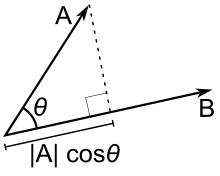
\includegraphics[width=0.30\textwidth]{dotproduct}
    \caption{A dot product in progress, as A is being projected onto B}
\end{figure}

Numerically, this projection is $|\vec{A}| cos(\theta) |\vec{B}|$, which corresponds to the length of the component of A that lies on B, times the length of B.

This definition derives some very useful other expressions, such as 

\begin{equation}
    \cos(\theta) = \frac{\vec{A} \cdot \vec{B}}{|\vec{A}||\vec{B}|}
\end{equation}
\begin{equation}
    comp_{\vec{B}} \vec{A} = \frac{\vec{A} \cdot \vec{B}}{|\vec{B}|} = \vec{A}\cos(\theta)
\end{equation}

Another way to define the dot product is the sum of the products of the components of the vectors. Another mouthful. The math is a easier to understand
\begin{gather*}
    \text{Let} \vec{A} = (A_1, A_2, ..., A_n)\\
    \text{Let} \vec{B} = (B_1, B_2, ..., B_n)\\
    \vec{A} \cdot \vec{B} = A_1 B_1 + A_2 B_2 + ... + A_n B_n
\end{gather*}
Let's call this the algebraic definition, as opposed to the projection or geometric definition from earlier.\\
This was surprising to me. How is this equivalent to the projection definition from earlier?
What helped me was realizing that this definition is equivalent to applying the geometric definition over the components of B.

\begin{gather*}
    \text{Let} \vec{A} = (A_1, A_2, A_3)\\
    \text{Let} \vec{B} = (B_1, B_2, B_3)\\
    \vec{B} = (B_1, 0, 0) + (0, B_2, 0) + (0, 0, B_3)\\
    \vec{A} \cdot \vec{B} =  \vec{A} \cdot (B_1, 0, 0) + \vec{A} \cdot (0, B_2, 0) + \vec{A} \cdot (0, 0, B_3)\\
    = A_1 B_1 + A_2 B_2 + A_3 B_3
\end{gather*}

This amounts to projecting A onto each component of B, which is just the corresponding component of A (projecting a vector onto a vertical vector is the same as taking the vertical component of the first vector and so on), 
multiplying their lengths, and adding all of those multiplications up, which gives us exactly the algebraic definition of the dot product


\subsection{Cross Products}
Cross products are, in my head, the counterpoint to a dot product. Whereas you can think of the dot product as what two vectors have in common (the component of one on another), the cross product gives the opposite, what the vectors do not have in common

Yet again we have two definitions, a geometric definition (again preferred by me), and an algebraic one

\textbf{Geometric Definition:} The cross product of two vectors ($\vec{A} \times \vec{B}$) is a new vector that is orthogonal to both vectors, whose length is equal to the area of the parallelogram formed by the two vectors being crossed.

\begin{figure}[h]
    \centering 
    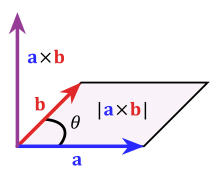
\includegraphics[width=0.30\textwidth]{crossproduct}
    \caption{The cross product}
\end{figure}

This seems a little strange. Why this definition of all things? It becomes a little clearer when we consider what the area of a parallelogram actually is.
This area is given by the base times the height, or for the vectors in the picture, $|\vec{A}| |\vec{B}|\sin(\theta)$, because $|\vec{A}|$ is the length of the base and $|\vec{B}|\sin(\theta)$ gives the height

So if the length of the cross product is this area, then $|\vec{A} \times \vec{B}| = |\vec{A}| |\vec{B}|\sin(\theta)$, and because we have introduced $\theta$, this becomes a very useful formula.

One use is to find the distance from a point and a line, which can be computed by crossing two vectors to form a parallelogram between the line and the point, and dividing by the length of its base to find the point's distance off the line.

It's worth specifically noting that the cross product returning an orthogonal vector is particularly powerful and useful. The length is arguably less useful of the two properties.

Actually computing this cross product is a little strange and unexplained to me, but I'll leave it here
\begin{align*}
    det
    \begin{vmatrix}
        \hat{i} & \hat{j} & \hat{k} \\
        A_1 & A_2 & A_3 \\
        B_1 & B_2 & B_3 \\
    \end{vmatrix}
\end{align*}

It's unclear to me why this produces an orthogonal vector, or why it is the length of the area of the parallelogram. Further research needed.

\subsection{Vector/Parametric Forms of Lines}

This is a short one. In $\mathbf{R}^2$, lines can be defined in point slope form. You start at a point, follow a slope, and you get your line. 
There's a similar concept in $\mathbf{R}^3$, with the vector form of a line. You start at a point, follow a vector, and you get your line.

The vector form of a line is as follows:
\begin{displaymath}
    L = \{\vec{r}(t) = P_0 + t\vec{d}\}
\end{displaymath}
Where $P_0$ is the point, and $\vec{d}$ is the direction vector of the line, the 3-space analog of a line's slope, and $t$ is some real number to scale the direction vector by.

This can also be rewritten in terms of each component of the vector that is returned by $\vec{r}(t)$, known as the parametric form of the line

\begin{gather*}
    x = P_{0x} + \vec{d}_xt\\
    y = P_{0y} + \vec{d}_yt\\
    z = P_{0z} + \vec{d}_zt\\
\end{gather*}


To compare to the other forms, all of the following draw the same line
\begin{gather*}
    y = x \\
    y - 0 = 1 (x - 0)\\
    L = \{\vec{r}(t) = (0, 0) + (1, 1)t\}\\
    \vec{r}(t)= (x, y): 
    \begin{cases}
        x = 0 + 1t\\
        y = 0 + 1t\\
    \end{cases}
\end{gather*}

As a sidenote, if you want to represent a line segement, instead of an infinite line, the idea is pretty cool. The line segement between two points starts at the first point and follows a vector formed by subtracting the points, and clamping $t$ between 0 and 1.

So the segment between $(a, b)$ and $(c, d)$ is represented by

\begin{gather*}
    \{\vec{r}(t) = (a,b) + t\left((c - a, d - b)\right)\}\\
    0 \leq t \leq 1
\end{gather*}

And checking this for $t = 1$ gives you 
\begin{displaymath}
    (a, b) + (c, d) - (a, b) = (c, d)
\end{displaymath}

And at 0 you get $(a, b)$, so the line will only exist between the two points. Pretty neat idea.

\subsection{Vector and 3D Functions}

Vector functions are pretty quick.
\begin{displaymath}
    \vec{v}(t) = (x(t), y(t), \dots)
\end{displaymath}

Their derivatives are the derivatives of the components of their vectors, and the usual derivative rules (product, quotient, etc.) work the way you would expect.

3D (or higher) functions are just as quick. Some function of x and y returns a z value, essentially taking the xy plane and raising it up along the z axis at each point $(x, y)$ to the value $f(x, y)$

If you want to take a derivative of these, you have to take some care, because there are now two axes in which you can move, so the notion of a derivative becomes a bit fuzzy. Enter the partial derivative

\textbf{Definition:} The partial derivative of a function is the derivative of a multidimensional function along a single axis. You take a slice of the surface created by the function, and the resulting single dimension of movement is the respect of the derivative. All other variables are treated as constants.

\begin{gather*}
    \frac{\partial}{\partial x}(f(x) = xy) = (1x^0)y \\
    \frac{\partial}{\partial y}(f(x) = xy) = x(1y^0)
\end{gather*}

\subsubsection{Tangent Planes and Linearization}
One of the uses of the derivative in 2 dimensions was to approximate a function. The tangent line is pretty close to the function at very small steps. In 3D, we need a tangent plane, to represent the two dimensions of movement we have.

To find a tangent line in $\textbf{R}^2$, we used a point and a slope $y - y_0 = f^\prime (x)(x-x_0)$. In $\textbf{R}^3$, we need two slopes, so 
\begin{displaymath}
    z - z_0 = \frac{\partial f}{\partial x}(x_0, y_0)(x - x_0) + \frac{\partial f}{\partial y}(x_0, y_0)(y - y_0)
\end{displaymath}
represents the tangent plane.

A little manipulation of that later and we get a way to linearize the function, which is pretty similar
\begin{displaymath}
    f(x, y) \approx f(a, b) + \frac{\partial f}{\partial x}(a, b)(x - a) + \frac{\partial f}{\partial y}(a, b)(y - b)
\end{displaymath}

Where $(a, b)$ is the point where you start, and $(x, y)$ is where you end up. Which amounts to starting at $(a, b)$, and walking a bit in the x multiplied by $\frac{\partial f}{\partial x}$, which is the slope (rise / run) in the x times the run, so you get the z that you should go up by, and you do the same in the y axis

We can think of tangent planes, tangent lines, and linearizations as applications of \textbf{differentials}. \textbf{Differentials} are generally linearizations of functions in whatever dimension the function is in. In two dimensions, the differential of a function is $dy = f^\prime (x)dx$, for any arbitrary dx. This gives you an equation for a tangent line. It's a slope times a change in the "run", so you get a rise.

In 3-space, the differential becomes slightly less clear because $f^\prime (x)$ now has to become partial derivatives. In 3-space $z$ changes instead of 2-space's $y$, but z can change in both the x and y axes. So to incorporate both of these, the total $dz$ will be dependent on $dz_x$ and $dz_y$.

We call then call $dz$ the total differential, defined by
\begin{gather*}
    dz = \frac{\partial f}{\partial x}(x, y)dx + \frac{\partial f}{\partial y}(x, y)dy  
\end{gather*}

This works out pretty well. When you bump x, what is the change in z. When you bump y, what is the change in z. The function that represents the total change in z is dependent on how much you bump x and y by. This then defines a tangent plane. You can bump x and y by any value, including zero, so this necessairly has to be a plane because it has to exist when either bump is zero, so it cannot be a line because it must be able to move independently in two axes. It also doesn't make sense to be a line. How are you going to represent two dimensions of potential change in a one dimensional object.

\subsubsection{Quadratic Approximation}
While we're doing linear approximations, we may as well touch on quadratic approximation.

Quadratic approximation approximates a 3D function as a paraboloid instead of a line. This is pretty useful, as it's a good idea to approximate a 3D function with a 3D figure, instead of 1D lines.

This approximation is just an extension of a taylor polynomial. It looks like:
\begin{displaymath}
    Q_f(x) = f(x_0) + \nabla f(x_0)\cdot(x-x_0)+\frac{1}{2}(x-x_0)^T\mathbf{H}_f(x_0)(x-x_0)
\end{displaymath}
That looks pretty scary, let's break it down.

First off, $f(x_0)$ is the value of the function at the point $x_0$. This is the y-intercept, so to speak, of the approximation, or the point at which we want to start the paraboloid.

To that, we add $\nabla f(x_0)\cdot(x-x_0)$. This is a linear term. It's a vector of partial derivatives dotted with a vector of changes in position from the point $x_0$. This will build a tangent plane. We add the change in z with a nudge in x, and the change in z with a nudge in y, together, to get the total z change at any point away from $x_0$, which will be rendered as a plane.

Finally, we add the scary quadratic term. The first thing we should break down is $\mathbf{H}_f(x_0)(x-x_0)$. $\mathbf{H}_f$ is the Hessian matrix of $f$, a symmetric and square matrix of second order partial derivatives.
We evalute $\mathbf{H}_f(x_0)$ to be those partial derivatives at $x_0$. We then multiply this matrix by a column vector of the same changes we had earlier. In 3D this works out as follows:
\begin{gather*}
    \mathbf{H}_f(x_0) = \begin{bmatrix}
        \frac{\partial f}{\partial xx} & \frac{\partial f}{\partial xy}\\
        \frac{\partial f}{\partial yx} & \frac{\partial f}{\partial yy}\\
    \end{bmatrix}\\
    \mathbf{H}_f(x_0) \cdot (x - x_0) = \begin{bmatrix}
        \frac{\partial f}{\partial xx}(x_0) \cdot (x - x_0) + \frac{\partial f}{\partial xy}(x_0) \cdot (y-y_0)\\
        \frac{\partial f}{\partial yx}(x_0) \cdot (x - x_0) + \frac{\partial f}{\partial yy}(x_0) \cdot (y-y_0)\\ 
    \end{bmatrix}\\
    \frac{1}{2}(x-x_0)^T\mathbf{H}_f(x_0) \cdot (x - x_0) = 
    [x-x_0, y-y_0] \cdot \begin{bmatrix}
        \frac{\partial f}{\partial xx}(x_0) \cdot (x - x_0) + \frac{\partial f}{\partial xy}(x_0) \cdot (y-y_0)\\
        \frac{\partial f}{\partial yx}(x_0) \cdot (x - x_0) + \frac{\partial f}{\partial yy}(x_0) \cdot (y-y_0)\\ 
    \end{bmatrix}\\
    = \frac{1}{2}\frac{\partial f}{\partial xx}(x_0) \cdot (x-x_0)^2 + \frac{1}{2}\frac{\partial f}{\partial yy}(x_0) \cdot (y-y_0)^2 + \frac{\partial f}{\partial xy}(x_0) \cdot (x-x_0)(y-y_0)
\end{gather*}

So what's this look like then? We have taylor polynomials along x and y, which makes sense. The third term is (kind of) a taylor polynomial along some combination of the x and y directions.

This is sufficient for any direction between the axes. If you consider how this is being computed, it's whatever change in x, and whatever change in y, times the "slope" when you move along a partial derivative. They aren't independent, though, they're multiplied. If they were independent this would be another linear term. Because they are multiplied, this will create a parabolic term. (Consider when the x change is identical to the y change to see this, you end up squaring the change)

This is all super shallow though, and I need to spend more time on it. Further research needed.
\subsubsection{Contour Maps}
\label{sssec:Contour Maps}
Before we leave 3D functions it's worth mentioning contour maps because they're cool.\\
\begin{figure}[h]
    \centering 
    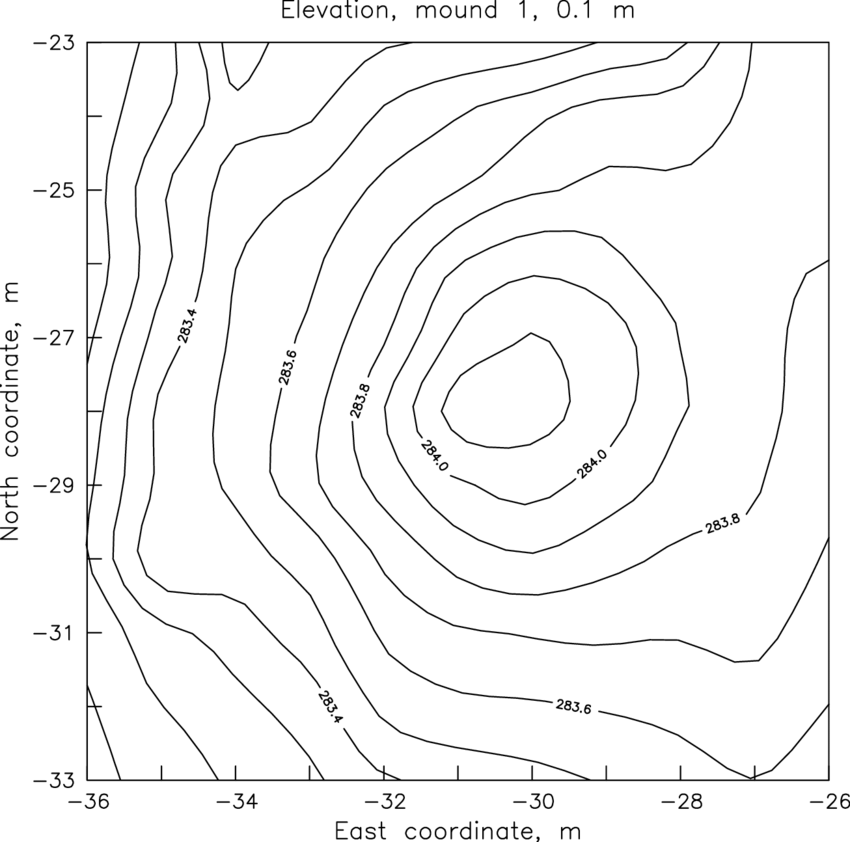
\includegraphics[width=0.5\textwidth]{contourmap}
    \caption{A contour map of some mound}
\end{figure}\\
The contour map of a 3D function is created by taking horizontal slices of the function at constant z values. This creates a neat way of visualizing these functions and will be useful for gradient fields later.

\newpage

\section{The Multidimensional Chain Rule}
What came before was all pretty clear the first time through. After this, though, was when the lectures started to get muddy, which inspired me to take some more detailed notes.

The multidimension chain rule is a weird one. I couldn't ever find a satisfactory answer, intuition, or explanation for why it made sense.

It helped to first consider the single dimension chain rule.

\begin{gather*}
    \text{For a function} f(g(x)), \text{Let } u = g(x) \\
    \frac{d}{dx} f(g(x)) = \frac{d}{dx} f(u) = f^\prime (u)\frac{du}{dx}\\
    \frac{du}{dx} = g^\prime (x)\\
    \frac{d}{dx} f(g(x)) = f^\prime (g(x)) g^\prime (x)
\end{gather*}

This is still pretty shallow for me. Seems more like a trick of notation than something that makes sense. If we go back and consider the derivative, though, it is definitionally the change in the value of the function when you change the input by a little bit.
\begin{gather*}
    f(x) = x^2\\
    f(x + dx) = (x+dx)^2\\
    = x^2 + 2xdx + {dx}^2\\
\end{gather*}

So when we nudge the input of the function by $dx$, we get $x^2 + 2xdx + {dx}^2$ as the height of the function at $x + dx$. Before the nudge, the function was $x^2$, so the nudge changes the function by adding $2xdx + dx^2$. As $dx \to 0$, the value of $dx^2$ becomes very small and much less significant than $2xdx$. So when we nudge the function, its return value meaningfully changes by twice the value of the function at x, times the tiny nudge we made in the x, meaning that $f^\prime (x) = 2x\ dx$. This is where the power rule comes from.

When we nudge $f(g(x))$, we first nudge $g(x)$ by something, and the new value then becomes the input of $f$.

Let's ignore $g(x)$ for a second. So long as $g(x)$ is differentiable, then a small change in x would feel no different than if we nudged $g(x)$, as far as $f$ is concerned. 
Let's call $g(x)$ $u$ instead. A small nudge in $u$, du, corresponds to a change of $f^\prime (u)\ du$. The nudge du is itself the change in $g$ when you change x, that nudge is $g^\prime (x)\ dx$, which gives us the chain rule

\begin{gather*}
    \frac{d}{dx} f(g(x)) = f^\prime (u)\ du\\
    du = \frac{du}{dx}dx = g^\prime (x) dx\\
    \frac{d}{dx} f(g(x)) = f^\prime (g(x)) g^\prime (x)\ dx
\end{gather*}

Okay, so with the single dimensional chain rule out of the way we still have a beast left. Let's look at something easy first.
\begin{gather*}
    \text{Let} f(a, b) = a + b\\
    \text{What is } \frac{\partial}{\partial x}f(x^2, y^3).
\end{gather*}

The first thing to note is that a and b are private variables. The user who is feeding x's and y's into f has only indirect control over a and b. This means that taking a partial derivative with respect to a or b means nothing here, because the user inputting variables only knows what x and y are, and has never heard of a and b

Now, if you're just looking at this, you can just plug the functions in.

\begin{gather*}
    f(x^2, y^3) = x^2 + y^3\\
    \frac{\partial f}{\partial x} = 2x \\
    \frac{\partial f}{\partial y} = 3y^2
\end{gather*}

So you dont actually \emph{need} the chain rule. You could plug all of the functions in and take a partial derivative as normal.
However, if your functions get complex, say $f(u, v) = u^2sin^2(v)$ and $u$ and $v$ are themselves complicated, the partial derivatives get annoying really fast, so having a way to pre-compute this with a formula would be nice.

Let's take that example. For $f(sin(x), cos(y))$ what happens when we nudge x? Let's again call sin(x) u.

\begin{gather*}
    f(u, \cos(y)) = u^2\sin^2(\cos(y))\\
    \frac{\partial f}{\partial u} = 2u(\sin^2(\cos(y))\ du\\
    du = \frac{du}{dx}dx = \cos(x) dx\\
    \frac{\partial f}{\partial u} = 2\sin(x)(\sin^2(\cos(y))\cos(x)\\
\end{gather*}

Okay, that's all fine and good I guess, but what does it actually mean? The first thing we did was ignore sin(x). We want a change in f with a change in x, but a change in x makes a change in u, so we considered the change in u first.
The change caused by u was $\frac{\partial f}{\partial u}$, which is some term times du. So what is du? We really want a change with respect to x, so how can we find du in terms of dx?
We can take $\frac{du}{dx}$, because u depends on the variable x, and then multiply that by dx, so that we're left with du.

So if $\frac{\partial f}{\partial u}$ is something times du, and du is $\frac{du}{dx} dx$, then $\frac{\partial f}{\partial x} = \frac{\partial f}{\partial u} \frac{du}{dx}$
This makes some sense. If we nudge x and it doubles u, and if we nudge u and it doubles f, it makes sense that nudging x quadruples f (by multiplying, not squaring/exponentiating).

This is nice, but what if v also depends on x? Then we also have to think about v now! So when we nudge x it makes some change to u, which makes a change to f, but it also makes a change to v, which makes a change to f. What's the total change?
Well u and v aren't really related. The function can do whatever it wants with u and v, but no matter what, when you take a partial derivative of one, the other is constant. Unless they're the same thing, but that's beside the point.
Because they create two independent changes, you just add them. You change x, it changes u, which changes f. It also changes v, which changes f. u and v don't change each other, so you don't multiply them or compose them or do anything fancy. The partial derivative is just the sum of the changes.

This is all honestly shallow intuition. I still don't really get all of this. My saving grace is this tree
\begin{figure}[h]
    \centering 
    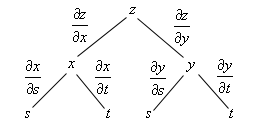
\includegraphics[width=0.5\textwidth]{chainruletree}
    \caption{How to compute a multidimensional chain rule}
\end{figure}

If you want \large$\frac{\partial z}{\partial s}$ \normalsize you follow all of the branches to s, multiply down the branch, and add the various branches. So,
\begin{gather*}
    \frac{\partial z}{\partial s} = \frac{\partial z}{\partial x} \frac{\partial x}{\partial s} + \frac{\partial z}{\partial y} \frac{\partial y}{\partial s}
\end{gather*}
This gives you what we had earlier. You keep unpacking various partial derivatives until you reach the variable you want, and then add all of the independent changes. I particularly like this tree becuase you could go 9 functions deep and it works the same way

My professor really likes emphasizing this derivative matrix $Df(x)$, which I think is supposed to be the \externalLink{https://en.wikipedia.org/wiki/Total_derivative}{Total Derivative} but everything about this seems like we'll get to it later so I'll skip it for now and instead focus on

\section{The Gradient and Directional Derivatives}
So first off, the gradient is, according to Grant Sanderson, weird. We'll start with the algebraic definition.

\begin{gather*}
    \nabla f(x, y, ...) = (\frac{\partial f}{\partial x}, \frac{\partial f}{\partial y}, \dots)
\end{gather*}

\begin{gather*}
    \text{Let} f(x, y) = x^2 sin(y)\\
    \frac{\partial f}{\partial x} = 2x\sin(y) \\
    \frac{\partial f}{\partial y} = x^2\cos(y) \\
    \nabla f(x, y) = (\frac{\partial f}{\partial x}, \frac{\partial f}{\partial y}) \\
    = (2x\sin(y), x^2\cos(y))
\end{gather*}

With this, it's important to note that the gradient is a \textbf{vector valued function}, which is a vector of all the partial derivatives of f. (Grant called this a full derivative, as it contains all of the partial derivatives).

A helpful way to think of this is
\begin{gather*}
    % \LARGE
    \nabla = \begin{bmatrix}
        \frac{\partial}{\partial x}\\
        \frac{\partial}{\partial y}\\
        \vdots
    \end{bmatrix}
    % \normalsize
\end{gather*}

And that $\nabla f(x)$ distributes $f(x)$ over that vector.

This is fine. It's a vector of partial derivatives, so what? What's neat about this is that it gives the direction of steepest ascent. That isn't at all intuitive at all, though. We just have a whole bunch of slopes in a whole bunch of directions. What gives?

First, a quick detour:

\subsection{Directional Derivatives}
What if instead of nudging a 3D function by x or y, we nudge it along some vector?
Pick some vector $\vec{v} = (a, b)$ to nudge along. This is like nudging by a in the x direction, and b in the y direction.
The directional derivative is
\begin{gather*}
    {\nabla}_{\vec{v}} f(x, y) 
    = a\frac{\partial f}{\partial x} + b\frac{\partial f}{\partial y} 
    = \vec{v} \cdot \nabla f(x, y)
\end{gather*}

Note the subscript of $\nabla$. Without it it's the gradient, as on the right, and with it it's the directional derivative.
Similar to a partial derivative, this corresponds to a slice of the graph of a 3D function from some plane that isn't necessarily parallel to either axis x or y.
That slice gives us some 2D function, where some step along that vector corresponds to a change in z, and some people write the directional vector as \Large $\frac{\partial f}{\partial \vec{v}}$ \normalsize to denote this.

That said, the line to remember is that the directional derivative is a partial derivative along some vector, instead of an axis. This is also results in giving you the slope of a graph when you walk along some vector, but you should be careful that when you are looking for the slope, you take a unit vector as the direction, otherwise you could get some multiple of the actual slope. 

Okay, with that in mind let's think about...

\subsection{Why the Gradient Gives the Direction of Steepest Ascent}

Imagine you are at a point on a 3D graph. In order to climb the graph as fast as possible, you want to find the largest slope from a directional derivative along some unit vector evaluated at your point. (A unit vector because $\vec{\infty}$ would always be the best choice)

To find this best vector, consider what the directional derivative actually is.

\begin{displaymath}
    \nabla_{\vec{v}} f(a, b) = \nabla f(a, b) \cdot \vec{v}
\end{displaymath}

If we want to maximize $\nabla_{\vec{v}} f(a, b)$, we really need to figure out what $\vec{v}$ dotted with $\nabla f(a, b)$ will give us the biggest slope (remember that $\vec{v}$ is a unit vector).

A dot product equals $|a| |b| \cos(\theta)$. When the vectors lie on the same line, ($\cos(\theta) = 1$) we get a maximal dot product, assuming $|a|\ \&\ |b|$ are fixed, which they are in a directional derivative.

Therefore, the best unit $\vec{v}$ will be on the same line as $\nabla f(a, b)$. It needs to be a unit vector, so take $\frac{\nabla f(a, b)}{|\nabla f(a, b)|}$ and you get a unit vector that returns the highest possible slope from a directional derivative

The gradient itself, evaluated at $(a, b)$, normalized, will then be the vector that, when traveled along, results in the greatest increase in altitude, because it is the highest slope, as we got from maximizing the directional derivative. Some more intuition is in the section on vector fields.

Pretty cool stuff. It's the backbone of the Gradient Descent Algorithm and I implemented it for a \externalLink{https://github.com/SAXTEN2011/LinearRegression/blob/master/index.js}{Linear Regression Model}

\subsection{Vector Fields}

Vector fields are pretty much what they sound like. It's a 2D plane of vectors, i.e. a function $f(x, y)$ that maps each point to some $\vec{v}$, which generalizes to some n-dimensional function mapping to some n-tuple

The construction of one such vector field can be done using the gradient operator. Taking $\nabla f(x, y)$ gives you some vector at the point $(x, y)$, and if you find the vector at every $(x, y)$ you get a vector field that we call the gradient field, because it was generated by the gradient operator. 

A neat thing to note is that the gradient field points in the direction of steepest ascent, because it is formed by the gradient. This is necessarily orthogonal to contour lines, as the steepest ascent is also the shortest path from one contour line to the next. If you zoom in super close on two nearby contour lines, they will eventually look like parallel lines. The shortest distance between parallel lines is an orthogonal path, so a gradient field will produce vectors orthogonal to a function's contour map.

\begin{figure}[h]
    \centering 
    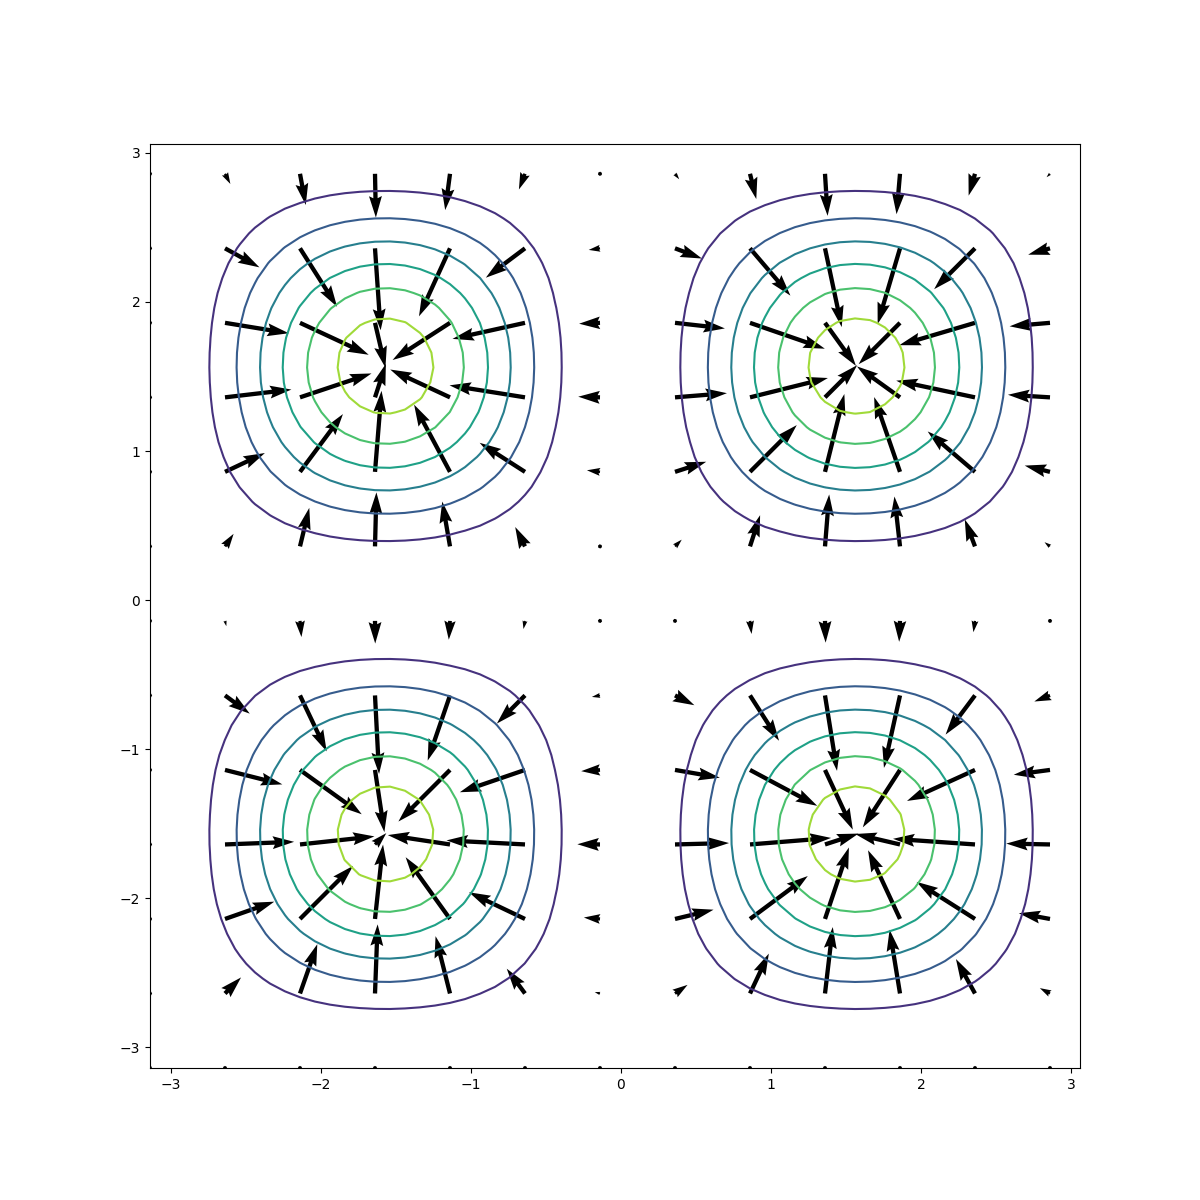
\includegraphics[width=0.75\textwidth]{orthogonalContour}
    \caption{A gradient field of $z = \sin(x)\sin(y)$ against its contour field. The vectors all point towards the peaks, which means orthogonal to the contours! Also, if they were parallel to the contours, you find a way to not ascend at all!}
\end{figure}

Okay so what. I get that being able to visualize a gradient field helps give some intuition for what following a gradient would mean, but why would I ever really need this outside of that intuition? 
The answer is on \externalLink{https://en.wikipedia.org/wiki/Vector_field\#Operations_on_vector_fields}{this wikipedia page} and I hope I take some notes on this. 
Further research needed.


\subsection{Tangent Planes to Level Surfaces}
If we want to find a tangent plane to a 3D surface, say $x^2 + y^2 + z^2 = 3$, we need to find some normal vector to the surface that we can make a plane from. To find this normal vector, we will be a little sneaky. We can think of this 3D function a level surface of a 4D function. A level surface is a slice in one axis of a function, so a level surface of a function, say $z = x^2 + y^2$, is just where $x^2 + y^2$ equals some constant $c$, i.e everywhere on the function that has a $z$ value equal to $c$, also known as a \hyperref[sssec:Contour Maps]{contour} of the function.

So we know that the gradient of a function points orthogonal to a contour line, because that is the fastest direction to the next contour line. Remember that the contour of a 3D function is some 2D curve, so the contour of a 4D curve is some 3D surface, and the gradient of a 4D function will result in a vector that is orthogonal to the 3D contour of the function. 

We can exploit this by thinking of some 3D surface as actually being some contour of a 4D function. So maybe we have some function $w = x^2 + y^2 + z^2$, in the 4D space defined by the axes x, y, z, and w. If we set $w$ to $3$, i.e take a level surface at $w=3$, then we get the sphere we led this section off with.

So to find a tangent plane to $x^2 + y^2 + z^2 = 3$, we should consider $x^2 + y^2 + z^2 = w$, a function of one higher dimension, and take a gradient. This will give a 3 vector that is necessarily orthogonal to the sphere because a 4D gradient will be orthogonal to its 3D contour. We can then use this gradient vector as the equation of a tangent plane $\vec{n}(p - p_0) = 0$, to find a tangent plane.

\section{Optimization}

In optimizing a function, we look for maximum and minimum values of the function. This is extremely useful across a wide range of use cases, the most prominent of which is probably machine learning.

\subsection{Finding Local Extrema}
In 2 dimensions this process is rather simple. You first find everywhere that the derivative is zero or undefined, so as to find points on the function where there is no direction you can move in to make your position better (whether better means a higher or lower altitude is up to you). You then check the second derivative of the function to see if the function is concave up (corresponding to a minima) or concave down (corresponding to a maxima).

In more than 2 dimensions we have the same general process. First we find where all partial derivatives are zero ($\nabla F(x, y) = \vec{0}$). If any of these partial derivatives weren't zero, then there would be a direction you could nudge the function in to increase or decrease the value of the function, thus your point is not an extrema. 
Put another way, the gradient points in the direction of steepest ascent, so if the gradient at a point is zero there is no direction that ascends, so you are at an extrema.
(Putting it this way sounds like it would only work at maxima. You can also get to minima by walking in the opposite direction to maxima, because the opposite direction of steepest ascent will be the steepest descent) 
It was surprising to me that the gradient being zero was sufficient. It seemed reasonable that your derivative in the X and Y could be zero but between those axes it wouldn't be. This is wrong though. If you take a directional derivative you dot the direction vector with the gradient. So if the gradient is zero, so are all of the directional derivatives. 

Once we find all of the critical points, we need to decide if these points are maxima, minima, or saddle points. To find this, we need a second derivative test.

To find the second derivative of a multidimensional function, let's find the derivative of the gradient. Each term will need to be derived with respect to every other element, so the gradient becomes a matrix,
\begin{align*}
    \nabla f &= \begin{bmatrix}
        \frac{\partial f}{\partial x}\\
        \frac{\partial f}{\partial y}
    \end{bmatrix}
    \xrightarrow{Becomes}
    \mathbf{H}_f = \begin{bmatrix}
        \frac{\partial f}{\partial xx} & \frac{\partial f}{\partial xy}\\
        \frac{\partial f}{\partial yx} & \frac{\partial f}{\partial yy}\\  
    \end{bmatrix}
\end{align*}

This matrix is called a Hessian Matrix, a symmetric matrix of the second order partial derivatives of a function. 
This is the equivalent of a second derivative of a multivariable function, and we can use it for a sense of concavity.
This will be very useful shortly.

If a critical point in 3D is a max or a min, the max/min will look like a paraboloid. If we find a taylor approximation of the 3D surface at a critical point, and the approximation looks like a paraboloid, then we know if it is indeed a max or a min, and its sign (whether the approximation is always positive or always negative) will distinguish between them.

We aren't really intersted in an accurate taylor approximation, we just want to try to fit a paraboloid to the surface and hope that it works. If it does work we've definitely got a max/min, and if it doesn't we almost certainly don't. Here's how we find this limited taylor approximation.

Firstly, we can linearly approximate the function. At any given point, the derivative with respect to some axis times the change in that axis will give a tangent line. In 3D we want a tangent plane instead of a line, so we dot the gradient with a vector formed by $(x, y, z) - p_0$, where $p_0$ is the point at which you are taking the derivative and $(x, y, z)$ represents some new position along each axis.

This spits out a plane, which tells us where the function is increasing and decreasing. At a critical point this must zero, because critical points necessarily have horizontal tangent planes, no increase or decrease as you nudge your coordinates.
We are doing this approximation specifically at critical points, so we can entirely ignore the linear part because of this.

So we look next at the concavity of the function, encoded by the second derivative. When you bump x, it changes the function's rate of change in the x proportional to it's second derivative.
If you take the new rate of change that the bump results in, and multiply that new rate of change by that bump again, you get the change in z caused by the second derivative.
It helps to think of this in units. If you are given acceleration, you need to multiply it by the time once to get a velocity, and again to get a position.
Meters per seconds squared, times seconds times seconds, gives you meters. In the same way, a second derivatives times a dx times a dx gives you a dz!

To represent this in 3D, we hit the hessian matrix on both sides with the change vector (in 2D we just multiply $f^{\prime \prime}$ by $(x - x_0)^2$). We've done lots of talking; here are some nice conscise symbols.

\begin{gather*}
    \text{Let } a = (x_0, y_0)\\
    f(x, y) \approx f(p_0) + \nabla f(p_0)(a - p_0) + \frac{1}{2}(a - p_0) \cdot \mathbf{H_f}(p_0)(a - p_0)
\end{gather*}
(the $\frac{1}{2}$ ensures that the derivative of the approximation is not twice the derivative of the actual function. 
This doesn't really matter in our case right now because it doesn't change the sign.)

But we only want to take this approximation at critical points, so $\nabla f$ is zero, and the linear term goes away!

So now our approximation is simply $f(p_0) + \frac{1}{2}(a - p_0) \cdot \mathbf{H_f}(p_0)(a - p_0)$

$f(p_0)$ is the height of the function at our critical point. If the second term is always positive, then we only add height when we move away from the point, so the critical point is a min, and if its a max then the second term must always be negative.

So now we can determine whether the function is a max/min by just looking at the sign of $(a - p_0) \cdot \mathbf{H_f}(p_0)(a - p_0)$, which is very nice!

So how do we find this sign? First let's figure out what that actually evaluates to.

After some multiplication that is both too long and too straightforward to write out, here is what we're left with in the 2 variable case
\begin{gather*}
    \frac{1}{2}f_{xx}(x_0, y_0)(x - x_0)^2 + f_{xy}(x_0, y_0)(x - x_0)(y - y_0) + \frac{1}{2}f_{yy}(x_0, y_0)(y - y_0)^2
\end{gather*}

That's pretty long. Because this is a quadratic form (i.e the product of two sums, for example $(a+b)^2$), let's write it as such.

\begin{gather*}
    ax^2 + 2bxy + cy^2
\end{gather*}
Where $a = \frac{1}{2}f_{xx}(x_0, y_0)$, $x = (x - x_0)$ and everything else follows in the same way.
(I think this is the first time I've used the $f_{xx}$ notation in these notes. This is equivalent to $\frac{\partial f}{\partial xx}$).

Note that we want to know where the \textit{evaluation} of the quadratic form is positive, not the slope or anything like that. 
We want to know this because we add the result of this to the height at our critical point. 
If the value of the approximation is always of the same sign, we can discern maxes and mins.

If a parabola (or paraboloid, but it's easier to consider 2D right now) is always positive, or always negative, it never crosses the x axis. A root of a function is definitionally when it crosses the x axis, so if this parabola has no solutions (or roots) then we know it is always the same sign and is definitely a min or a max.

But we're trying to approximate a 3D function, so we need to consider paraboloids for approximation, not parabolas. Thankfully, if a paraboloid crosses the x axis, then the slice of the paraboloid where y is some constant value where that crossing happens, then the resulting parabola from the slice will also have a root at the same place.

So to figure out if a paraboloid has a root, let's fix $y$ to be some $y_0$, so our quadratic form is now
\begin{gather*}
    ax^2 + 2bxy_0 + c(y_0)^2
\end{gather*}
So now we have a parabola (because it's only a function of a single variable, x, now), parameterized by some $y_0$. If we can't find a $y_0$ that gives this quadratic form roots, then we must have a max or a min, because no roots means not crossing the x axis which means the parabola is only positive or only negative.

Alright, let's find these roots then. Enter the old quadratic equation.

\begin{gather*}
    \frac{-2by_0 \pm \sqrt{(2by_0)^2 - 4ac(y_0^2)}}{2a} \\
    =\frac{-2by_0 \pm \sqrt{y_0^2 (4b^2 - 4ac)}}{2a}\\
    =y_0\left(\frac{-2b \pm 2\sqrt{b^2 - ac}}{2a}\right)\\
    =y_0\left(\frac{-b \pm \sqrt{b^2 - ac}}{a}\right)\\
\end{gather*}

This equation returns x values of solutions. If this value is not real, there aren't any solutions. This formula will never be real if $b^2 - ac$ is negative, because the square root of a negative is imaginary.

The obvious problem here is when $y_0$ is zero. This is problematic because it smooths over other solutions. If there was also a root at, say, $x=1$, it would get multiplied by zero, so the test will be inconclusive.

If the test is conclusive (i.e. $y_0$ isn't 0), we return back to needing to know when $b^2 - ac < 0$, in order to find when our paraboloid has no real solutions. We're pretty abstracted now, so let's fill back in a, b, and c with their actual values.
\begin{gather*}
    b^2 - ac = (\frac{1}{2}f_{xy})^2 - (\frac{1}{2}f_{xx} \cdot \frac{1}{2}f_{yy})\\
    = \frac{1}{4}f_{xy}^2 - \frac{1}{4}f_{xx}f_{yy}\\
\end{gather*}

So now we want to find when $\frac{1}{4}f_{xy}^2 - \frac{1}{4}f_{xx}f_{yy} < 0$. This is equivalent to
\begin{gather*}
    f_{xy}^2 - f_{xx}f_{yy} < 0 \\
    f_{xx}f_{yy} - f_{xy}^2 > 0
\end{gather*}
We make these changes because it puts the statement exactly in the form of the determinant of the Hessian matrix! That's pretty crazy. The determinant of the hessian will determine if a quadratic approximation at a critical point does or does not have solutions. If the approximation has no solutions, then the paraboloid is always positvely or negatively valued, and thus is a max or a min.

We can finally determine whether this is actually a max or a min by looking at either of $f_{xx}$ or $f_{yy}$. We know with absolute certainty that this point is either a max or a min,
and as a result know that the approximation at this critical point is a paraboloid. A paraboloid can't have one concavity in one axis and a different concavity in another,
so looking at either second order partial derivative will tell us directly if the paraboloid is concave up, or concave down, and we can then make the final call whether a critical point is a max or a min.

Okay, okay, that was super long. Let's recap.
We have a function and want to know where the local maxes and mins are.
These will happen at critical points ($\nabla f = \vec{0}$), but we need to figure out if each critical point is a max or a min.
To find out if it's a max or a min, we will try to approximate the function with a paraboloid.
If that paraboloid is always positively valued we have a min, and oppositely for a max.
That paraboloid can't always be positively valued if it crosses the xy plane.
We can find where that paraboloid crosses the xy plane by finding the solutions to the paraboloid.
We can find these solutions from the quadratic formula, and because the quadratic formula takes a square root of $f_{xy}^2 - f_{xx}f_{yy}$, we can force the paraboloid to not have solutions if that value is negative.
That value just so happens to be the \textbf{negative} determinant of the hessian matrix, so the opposite sign of the determinant of the hessian matrix is also the sign of the bit under the square root of the quadratic equation.
If the determinant is positive, then the bit under the square root is negative.
Negative square roots aren't real, so the paraboloid has no solutions, therefore never crosses the xy plane, therefore is always positively valued (or always be negatively valued), and we must really have a min (or a max)!

The textbook will not write all of that out, and will just give the following rule:
\begin{enumerate}
    \item If the determinant of the hessian is positive, then the sign of $f_{xx}$ tells you whether it's a max or a min.
    \item If the determinant is negative, then we have a saddle point (because there's a crit point but it isn't a max or a min)
    \item If the determinant is zero, the paraboloid might have solutions, who knows, so the test is inconclusive.
\end{enumerate}
To elaborate on point 1 a bit, if the determinant of the hessian is positive, the paraboloid has no solutions. 
If the paraboloid has no solutions, then it never switches sign. 
Because it never switches sign no matter what, all points near the paraboloid have the same concavity.
If they didn't, the approximation wouldn't have worked out to have no solutions.
We fit this paraboloid based on the partial derivatives, so we knew from the start it would follow their concavity, but we didn't know if everything else between them agreed, or even if they agreed themselves.
When the paraboloid has no solutions, every direction from the critical point has the same concavity, so we can just pick any one of those directions to figure out if we're at a min or a max.
For some reason conventions says to pick xx, but you could just as easily pick yy.
No matter which direction you pick, a positive value means a min, and a negative value means a max.
\subsection{Finding Absolute Extrema}
When we look at critical points and second derivatives we are finding local extrema, places on the function where there are no bumps to your input you can make to gain or lose altitude.

If we want to look for the highest point anywhere on the curve, the absolute maximum (or minimum), we need to do some thinking first.
For example, what's the absolute maximum of $f(x) = sin(x)$? Well there are a lot of them. Infinitely many of them, actually.
What if we wanted to know the absolute maximum and absolute minimum values of $f(x) = \frac{1}{x}$? This is even less clear.
Is infinity a value? Is that the absolute max and negative infinity is the absolute min? If so, at what x value do those extrema happen at?
It's not zero, but any value that's not zero can always get a little closer to zero, and increase the altitude of the function, and therefore can't be an extrema.

It would really help if we just said that we want to find the absolute extrema on some closed interval.
When we consider the absolute extrema in some interval, there are two places we can find these extrema.
First, the critical points will give us local maxes and mins. 
These maxes and mins may well have the biggest or smallest height of the function at their points, but we aren't guaranteed this.
If you chop the function off at the end of some interval, you could chop it off at some really big value that would have kept getting bigger outside of the interval
(For example, chopping $x^2$ at any value outside of zero will put absolute maxes at the endpoints of the interval). 
But these chopped points won't be critical points, because they weren't local extrema, just large values that would have been larger outside of the bound.
We need to specifically look for these points when searching for absolute maximum/minimum values because they won't show up when we solve for critical points.

So to find the absolute extrema of a function, we take all of the critical points, and all of the endpoints of our closed interval, and find the biggest and smallest values among them.
We actually don't even need to check whether the critical points are actually local maxes or mins. We can just find all of their values and take the biggest and smallest.
We might as well just evalute the function at the critical points instead of dealing with second derivative tests.
We are, after all, looking for the biggest and smallest heights of the function.
Who cares if that happens at a saddle point or not.

In 2D evaluating a function at the endpoints of an interval is super easy. If the interval is $[0, 1]$, then you just take $f(0)$ and $f(1)$.
In 3D, life isn't as easy\footnote{Is it ever?}.
We need to slice the surface along some direction or curve or whatever defines our interval.
So maybe the interval we care about is the unit circle (points with distance 1 from the origin), or a square from $(0, 0)$ to $(1, 1)$.
In each of these cases, we need to take some kind of slice of the function, which will give us a 2D function and then find the absolute extrema on that 2D function!
So there you have to find the critical points of the 2D slice, evaluate it at its endpoints, and it's a real pain.
This all sounds like I'm leading up to some nice trick. I'm not. I hope there's a better solution out there though.
Further research needed.

So the overall process for finding 3D absolute extrema goes as follows:
\begin{enumerate}
    \item Find the critical points
    \item Find any suspicious points on the boundary of the interval
    \item Evaluate the function at all of the points you collected from the first two steps. The biggest and smallest values are your absolute extrema.
\end{enumerate}
The suspicious points are places on the boundary of the interval that might be extreme values.
The boundaries are 2D slices of the function, so you should just find the absolute max/min on that 2D slice, and throw that in the pot with the critical points of the surface inside the interval.
Finding absolute extrema then becomes a nested problem.
You need to consider all of the extreme values within the 3D surface bounded by the interval \emph{and} all of the extreme values on the 2D boundary slices. 

\subsection{Constrained Optimization}
This is the form of optimization that makes up all the fun word problems.
You're always either building a box with maximal volume and a fixed amount of cardboard,
or the biggest pen for your cows with a fixed amount of fence.

Whatever the random problem the professor came up with is, you need to find the optimal inputs given some constraint.
The textbooks, in an effort to make you work as hard as possible, call the function you want to optimize f, and the constraint function g.
This was frustratingly abstract to me. The idea is pretty obvious, but is obscured by notation.

What was strangest to me was the notion of a constraint function.
The easiest example of a constraint function is representing how much cardboard you have to build a box.
If L, W, and H, are the length, width, and height of the box, then your constraint function might look like
\begin{gather*}
    g(L, W, H) = 2LW + 4WH
\end{gather*}
Which represents twice the cardboard to make the base, and 4 times the cardboard to make a wall.
In other words, the amount of cardboard it takes to build you box.
So why can't you just say that you only have 12 square feet of cardboard and not bother with this function?
It's actually a useful construction.

If you take a level surface of $g$ at 12, that represents having only 12 square feet of cardboard.
If you plug in your L, W, and H, to $g$, it tells you if you are within the constraint.
If you use 5000 square feet of cardboard, that doesn't equal 12, and your constrait function will be a contradiction. 
Put another way, if you find some optimal point on $f$, and that point isn't on the level curve of $g$, then you can't use that point.
This lets us reduce our problem to finding the absolute maximum value on $f$, constrained to points on $g$.

But this isn't so clear. We take a level surface at $g = 12$ (12 is just some random value that I'm taking for an example),
this level surface is 2D. That can't really intersect with $f$, which is a 3D surface.
It can, however, intersect with contour lines of $f$.
We could also just say that we care where the x and y values of points on f are also points on g,
or even say that we extend the level surface of g to be a cylinder so that we can find meaningful intersections,
but thinking about it as a contour map is a really useful perspective. 

When a level surface of $g$ (which I am going to just call $g$ from here on out) crosses a contour line of f we can figure out a couple of things.
First, we know that the point at which they intersect is a candidate for the optimal point.
This is because the point at which they intersect is necessarily on f and g, and we are trying to find the optimal point that satisfies exactly this fact.
However, we can also immediately disqualify this point!
If $g$ \emph{crosses} a contour line of $f$ it must be moving to another contour line somewhere else.
This value \emph{has} to be bigger or smaller than the point at which the lines crossed, because if the new value wasn't different than the value at which we crossed the contour line, then it would have to be on the contour line.
But it isn't on the contour line because we crossed the contour line, so we're moving to bigger and better places if we follow $g$, so we keep following $g$.
When do we stop then? If $g$ just barely touches a contour of $f$, i.e $g$ is tangent to a contour of $f$, then $g$ is always less than (or greater than) the value of that contour line, except when $g$ touches that value, in which case it is a local optima!
That's huge news! When $g$ is tangent to a contour of $f$, we find a local optima. So let's just find all of those local optima, evaluate the function at all of the points, and pick out the best value.

We can find these by considering what it means for two curves to be tangent to each other. 
The tangent line of the curves must be parallel, and the curves must share a point.
If they don't share a point, they can't be tangent, and if their tangent lines at the point that they share aren't parallel, then you could follow the tangent line to get inside of the other curve.
The curves being tangent means that you cannot do that. 
Put another way, the tangent line is a linear approximation. 
If the linear approximation of both functions are parallel, the functions don't cross over into each other. 
I am having a difficult time justifying this fact and \textbf{need to rewrite it}.

So where are tangent lines to contour maps parallel? 
Well first off, how do we even get tangent lines to contour maps?
The gradient will spit these out, as we talked about earlier on in the notes.
So now we just need to find where the gradient vectors of $f$ and $g$ (the function, not the level surface at 12), are parallel.
Vectors are parallel if one is a multiple of another, so we can express this as
\begin{gather*}
    \nabla f(x, y) = \lambda \nabla g(x, y)
\end{gather*}
Where solutions are the critical points of the function.
This might not be enough information.
Frequently we can solve for lambda, but not x or y.
In order to solve for x or y, we can also go back to our constraint function, and consider the system
\begin{displaymath}
    \begin{cases}
        \nabla f(x, y) = \lambda \nabla g(x, y) \\
        g(x, y) = 12
    \end{cases} 
\end{displaymath}
It's important that this system also has the constraint function in it, because it constrains solutions to only those that satisfy g.
If you only looked at $\nabla f(x, y) = \lambda \nabla g(x, y)$, you could find solutions well outside the constraint.
Because $g$ equals some constant, we can find x or y in terms of lambda, plug the lambda value into $g$, and solve for the other variable, which will be a definite value.
Then we have cocnrete values for x and y, evaluate the function at that point, and find the maximum and minimum values between those to find our absolute extreme values.

\subsection{Constrained Optimization With Two Constraints}
The process is almost exactly the same, except that it takes the following form:
\begin{gather*}
    \nabla f(x, y) = \lambda \nabla g(x, y) + \mu \nabla h(x, y)
\end{gather*}
Where $g$ and $h$ are constraint functions. My big question was "why addition?"

Wikipedia's article says to consider the constraint functions to be two lines.
The intersection of those lines will be the only point that satisfies both constraints, and will thus be the max.
However, these lines can't share a tangent line to each other (they wouldn't intersect), so it can't be possible that contours f, g, and h, all share a tangent line, which is what I initially thought multiple constraint solving would look like.
In this case, the gradient of f needs to be some linear combination of the gradient of the other two constraints, and multiple constraints generalize in the same way.

Further research needed as to why this makes sense.

\section{Multiple Integrals}
In 2D we can find areas under curves with integrals, and that's super useful!
For example, I used it in some functions for rewriting \externalLink{https://github.com/SAXTEN2011/GyroLib2020}{GyroLib} to find theta from angular velocity.
It's really useful to be able to climb up the position/velocity/acceleration tower, in the same way that it's useful to go down it with derivatives.

In 3D we look for volumes under surfaces, instead of areas under 2D curves.

From 2D, we added a whole bunch of rectangles of height $f(x)$ and width $dx$. 
In 3D, we use rectangular prisms of height $f(x, y)$, length $dx$ and width $dy$.

Another nice way to do this is to add up areas under slices of the surface. 
We can fix some y value to $y_0$ and take the corresponding slice of the function.
Integrating this 2D function gives us the area of that slice.
If we now consider $y_0$ to be the variable $y$, we can integrate that integral over y.
This adds up the areas of all of the slices of the functions, and gives us a volume.

Given that adding up slices in the x or slices in the y measures the same volume, the order of integrating doesn't really matter, except when it does.
Fubini's Theorem dictates when it matters, but it's not super relevant right now.
Everything we're given to compute in class will work just fine both ways.

To actually compute multiple integrals, you perform something called...
\subsection{Iterated Integrals}
Iterated Integrals are how we actually find the volume under a surface.
Let's look at an example
\begin{gather*}
    \int_c^d \int_a^b f(x, y) \,dx\,dy
\end{gather*}
To compute this, you take $\int_a^b f(x, y) \,dx$ and compute it. We'll call the result $u$.
You then compute $\int_c^d u\,dy$ to find the final volume.

Here's an example with numbers!
\begin{gather*}
    \int_0^1 \int_0^1 (x+y) \,dy\,dx\\
    = \int_0^1 xy + \frac{1}{2}y^2 \biggr \rvert_0^1 \,dx\\
    = \int_0^1 x + \frac{1}{2}\ \,dx\\
    = \frac{1}{2}x^2 + \frac{1}{2}x \biggr \rvert_0^1\\
    = \frac{1}{2} + \frac{1}{2} = 1
\end{gather*}

\subsection{Integrating Over a General Region}
Sometimes we want to integrate over nicely shaped domains like rectangles.
This is pretty straightforward.
Sometimes we want to integrate over crazy squiggly lake shaped things.
This is not so straightforward.

When we integrate over some region (say between two sine waves, i.e $sin(x)$ and $sin(x) + 5$ we might actually have to be mindful of our integrals.
If we take vertical slices of our domain, we're fine.
Horizontal slices, however, could intersect the sine wave, and all of the sudden our integral is way off.

In these cases, we need to consider the shape of the function to make sure we are taking slices of the function that make sense.
This is like performing the vertical line test.
If we pass a horizontal (or vertical) line across the domain, and intersect the domain in a nontrivial way, we can't take slices in that direction.

The way to figure out what direction is to just visualize the domain. 
It's not that hard to see which axis will give you trouble. 
The more tricky part is knowing if your problem axis goes first or second.
Remember that the outside integral is what adds up slices, so if you're going along the y axis to add slices (i.e your outside integral is w.r.t y), then you must be adding up slices that are parallel to the x axis.
Similarly, if you are adding up slices as you move along the x axis, you must be slicing in the y direction.
So your slice direction is the inside integral, so that the outside integral moves orthogonal to that direction to compute a volume.
\textbf{Problem axes become outside integrals.}

Hold on. What if I want to integrate over a square whose edges are sine waves?
Every axis is a problem axis!

If at all possible, try not to want to do this. However, here is how you would do this.

Just like in 2D, you can add integrals together to get areas,
so the integral from 0 to 1, plus the integral from 1 to 2, is the same as the integral from 0 to 2, assuming no funny business.
In 3D we have the same principle. If you integrate over two adjacent domains, and add their integrals, it's like integrating over both of them in one step.
So now just split your square into a whole bunch of domains that have only a single problem axis (maybe one domain between the top and bottom sine wave, one domain as the area of the left sine wave and a third as the area of the right sine wave).

You also could do some thinking about whether the sine waved sides change the area or not.
If they cover a full period it might be identical to a normal square with lines as sides.
Frequently, you can think about properties like that (frequently symmetry as well) to cheat the integral a bit.

\subsection{Changing Order of Iterated Integrals}
For some reason, you might want to change the order of iterated integrals. 
Maybe the math is easier when you integrate x first, and then do y, or maybe it's easier the other way around.

If you're integrating over some strange bounds, pretty much anything but a rectangle, the process isn't so easy.
Say you want to integrate over some squiggly shaped domain.
You need to take slices of the function in a different direction, which will require new bounds to be computed.

For example, the problem axis in figure 6 is the x axis.
\begin{figure}[h]
    \centering 
    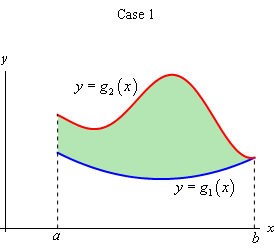
\includegraphics[width=0.5\textwidth]{problemaxis}
    \caption{}
\end{figure}
It might be easier to think of it as the problem direction, instead of an axis, but whichever way you think about it, you want to take vertical slices.

How do you take a vertical slice? 
You integrate with respect to y!
That tripped me up a lot. If you integrate with respect to x in 2D you get slices parallel to the y axis.
So what gives? Why does integrating w.r.t y in 3D produce vertical slices of the function all of the sudden?
When you integrate w.r.t y in 3D, you hold x to be a constant. This gives you a 2D function in the yz plane.
The base of that graph is the y axis, so you end up slicing the domain of integration along the y axis as well.
That slice is represented as:
\begin{gather*}
    \int_{g_1(x)}^{g_2(x)} f(x, y) \,dy
\end{gather*}
You then apply your outside integral over x to add up all of those y slices.
\begin{gather*}
    \int_a^b\left(\int_{g_1(x)}^{g_2(x)} f(x, y) \,dy\right)\,dx
\end{gather*}

A final way to see this is that the domain is between two functions of x. 
If you try to integrate that with respect to x, the bounds \emph{and the function} depend on x, and that is potentially impossible?
Just avoid all of that by integrating w.r.t y first
\end{document}